\chapter{Introdução}
%\markboth{\thechapter ~~~ Introdução}{}
%\label{intro}

Um sistema pode ser visto como um processo com sinais de entrada que são 
transformados ou induzidos a responder de alguma forma resultando em outros 
sinais de saída \cite{Oppenhein}. O intuito do controlador é manipular o sistema com a 
finalidade de obter um sinal de saída que siga uma referência pré estabelecida. Para isso, 
é necessário, primeiramente, obter um modelo que descreva 
o comportamento do sistema e, em seguida, projetar uma estratégia de controle a 
partir desse modelo. Dentre as técnicas utilizadas para modelagem cabe destacar a 
descrição do sistema por meio de equações diferenciais lineares \cite{Ogata}
ou a identificação de subsistemas \cite{Aguirre}.

No controle em malha aberta, a saída não exerce nenhuma influência sobre o sinal de 
controle. Dessa forma, um sinal de controle é aplicado à entrada de uma planta ou 
de um processo de modo que a variável controlada atinja um valor pré-estabelecido; 
entretanto, esse valor resultante na saída não é utilizado para modificar a entrada. 
O problema deste tipo de controle é que o sistema pode mudar seu ponto de operação
, por exemplo, ao ocorrerem perturbações. Caso isso ocorra, a saída não 
terá o valor estabelecido anteriormente.

Ao fechar a malha, o sinal de saída passa a influenciar diretamente a ação de 
controle. Assim, o sistema passa a contar com uma malha de realimentação e o sinal 
observado na entrada do controlador é, agora, o erro entre a referência do sistema e 
a saída mensurada. O controlador, então, tende a minimizar o erro de modo a garantir 
que a saída do sistema seja igual a referência, como ilustrado na \autoref{fig:diagBloco}.
``Controlar a saída de uma planta ou de um processo por realimentação significa aplicar 
na sua entrada, após conveniente amplificação, o sinal resultante da 
diferença entre o valor desejado e o valor medido da saída \cite[p.~3]{Castrucci}.''

O controle em malha fechada utiliza a informação de como a variável controlada evolui 
para determinar o sinal de controle aplicado ao processo. Determinado o modelo da 
planta a ser controlada, o controlador é sintonizado de forma a atender especificações 
de projeto fornecidas, tais como: sobressinal máximo, tempo de acomodação, tempo de subida
e a constante de tempo (no caso de sistemas de primeira ordem). Geralmente, 
uma vez sintonizado o controlador e validado seu desempenho em malha fechada da 
planta realimentada, passa-se à implementação prática do controle sem que haja 
uma prévia validação do comportamento do controlador quando implementado em 
dispositivo físico.

Uma das formas de se controlar uma planta é através da inclusão de um hardware real na malha
de controle. Essa é a idéia básica da simulação \emph{Hardware in the Loop} (HIL), uma técnica
bem estabelecida usada em projeto e avaliação de sistemas de controle \cite{Bacic}.

Essa técnica consiste em implementar um controlador previamente projetado e validado em um dispositivo físico e 
substituir o bloco de controle $C(s)$ (vide \autoref{fig:diagBloco}) por esse dispositivo, como apresentado na 
\autoref{fig:diagBlocoHIL}. Ou seja, o sinal de erro $E(s)$ é transmitido para um dispositivo físico externo, 
o qual é responsável por determinar a ação de controle a ser aplicada ao modelo da planta em estudo $G(s)$. Em seguida, o 
sinal de controle calculado é enviado de volta para o ambiente de simulação, no qual a saída $Y(s)$, teórica, 
é determinada. O intuito é verificar se a estratégia de controle e o desempenho associado permanecem 
adequados antes de realizar o controle diretamente na planta real.

\begin{figure}[ht]
  \centering
  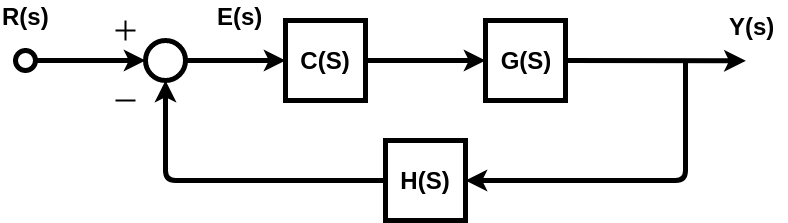
\includegraphics[width = 0.6\columnwidth]{Imagens/blocosMF.png}
  \caption{Diagrama de blocos do sistema em malha fechada}
  \fonte{Do autor}
  \label{fig:diagBloco} 
\end{figure}

\begin{figure}[ht]
  \centering
  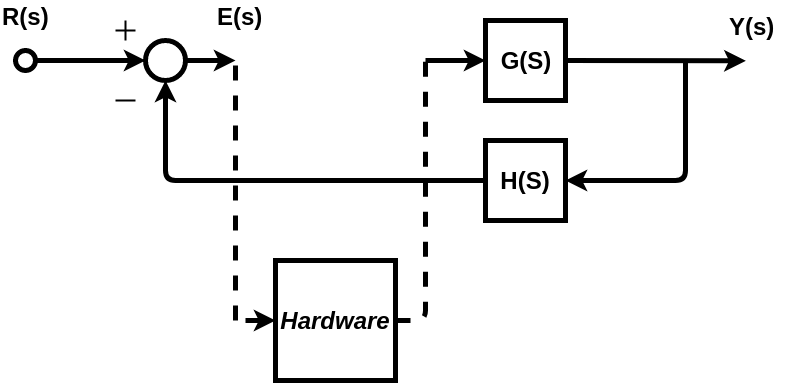
\includegraphics[width = 0.7\columnwidth]{Imagens/blocoHard.png}
  \caption{Diagrama de blocos do sistema em malha fechada - \emph{Hardware in the Loop}}
  \fonte{Do autor}
  \label{fig:diagBlocoHIL} 
\end{figure}

A metodologia para síntese do controlador, validação e implementação na planta real possui
três etapas distintas de execução. A etapa um consiste em levantar o modelo da planta que 
pretende-se controlar, e depois sintonizar um controlador em ambiente de simulação que atenda
às condições de projeto previamente especificadas. A segunda etapa propõe substituir 
o controlador virtual por sua implementação em dispositivo físico e validar a implementação 
em conjunto com o ambiente de simulação. Por fim, a etapa três consiste na utilização do controlador
implementado no dispositivo físico comunicando diretamente com a planta real.

\section{Motivação e Justificativa}
\markright{\thesection ~~~ Motivação e Justificativa}
%\label{motiva}

Quando os processos possuem uma dinâmica mais rápida que a execução do algoritmo para a ação 
de controle, surge um problema computacional complexo. Cumprir a restrição de reduzir o tempo
de resposta exige um uso maior de simulações em tempo real \cite{Isermann}. Nos sistemas de 
tempo real, as tarefas consideradas críticas devem executar dentro de um período de tempo 
estabelecido. A utilização de um \textit{Hardware} em uma malha de controle, conforme o 
método HIL propõe, possui um ganho em relação às simulações com 
sistemas operacionais comuns pelo motivo exposto acima.

Atualmente, as simulações HIL são utilizadas mais recorrentemente
para o desenvolvimento de novos componentes e atuadores em vários campos
diferentes \cite{Bouscayrol}. As aplicações ao longo da história têm demonstrado a 
variabilidade do uso da metologia, aplicações estas como, sistemas eletrônicos de 
potência \cite{Rothstein}, sistemas de controle de voo \cite{Karpenko}, engenharia 
de tráfego \cite{Bullock} e robótica móvel \cite{Kamali}.

% A ação de controle agora não depende 
% apenas da computação numérica, mas também da forma como o modelo interage com um 
% equipamento de controle externo. Além disso, o conceito de sistemas embarcados 
% exige cada vez mais o uso de ferramentas independentes encarregadas de executar 
% uma função específica.

% Sabe-se que os seres humanos têm limitações para frequentar determinados ambientes, 
% principalmente os ambientes industriais, onde estão submetidos à alta insalubridade 
% \cite{Lacaz}. Consequentemente, nos últimos anos, tem sido cada vez mais frequente 
% em indústrias, o uso de tecnologias que visam automatizar seus processos de 
% fabricação. Essas soluções visam a melhoria na qualidade do trabalho, e, 
% consequentemente, um aumento de produtividade. Os manipuladores robóticos são 
% exemplos de soluções deste tipo, sejam eles controlados remotamente, ou totalmente independentes 
% da ação humana. A maior parte das aplicações de manipuladores está voltada para a indústria, 
% principalmente as que utilizam linhas de produção, como montadoras e fabricantes de autopeças
% \cite{Spong}.

\section{Objetivos do Projeto}
\markright{\thesection ~~~ Objetivos do Projeto}
%label{objetivos}

O objetivo principal do presente projeto é sintonizar e validar estratégias de 
controle para o sistema dinâmico de um manipulador robótico utilizando a técnica 
\emph{Hardware in the Loop} (HIL).

\section{Local de Realização}
\markright{\thesection ~~~ Local de Realização}
%\label{empresa}

Departamento de Engenharia Eletrônica da UFMG (DELT/UFMG). O departamento 
situa-se dentro do campus Pampulha da UFMG na Escola de Engenharia. O campus 
fica na Av. Presidente Antônio Carlos 6627 - Pampulha, Belo Horizonte - MG, 
31270-901.

O departamento foi criado em 1969 e tem contribuído para a formação dos 
engenheiros eletricistas e engenheiros de controle e automação da UFMG. O DELT é 
referência no cenário nacional e é, também, o Departamento da UFMG com maior 
participação no curso de graduação em Engenharia de Controle e Automação.

\section{Estrutura da Monografia}
\markright{\thesection ~~~ Estrutura da Monografia}
%\label{organizacao}

A monografia está dividida em cinco capítulos. Este capítulo apresentou uma introdução 
ao projeto e o local onde o trabalho foi realizado. O Capítulo 2 faz uma revisão 
bibliográfica sobre os principais temas trabalhados no decorrer do projeto, como a modelagem e
controle de sistemas dinâmicos lineares, os conceitos da técnica \emph{Hardware in the Loop} (HIL)
e os princípios básicos do manipulador robótico. O Capítulo 3 aborda a metodologia de desenvolvimento
do trabalho, ele descreve como o projeto foi desenvolvido explicitando o passo a passo
das tarefas executadas para que o mesmo fosse concluído. Os resultados experimentais são 
apresentados no Capítulo 4: primeiramente, o modelo da planta é obtido, depois um controlador é modelado
em ambiente de simulação, o controlador é aplicado em um dispositivo físico para controlar a planta 
simulada, e por fim, a planta simulada é substituída pela planta real.
Finalmente, no capítulo 5, tem-se a conclusão da monografia com algumas sugestões 
para trabalhos futuros e dificuldades encontradas na realização do projeto.


\clearpage